\subsection{Point and Multi-point Kinetics}
\begin{frame}
        \frametitle{PyRK: Python for Reactor Kinetics}

               \begin{figure}[t]
                \vspace*{-0.1in}
                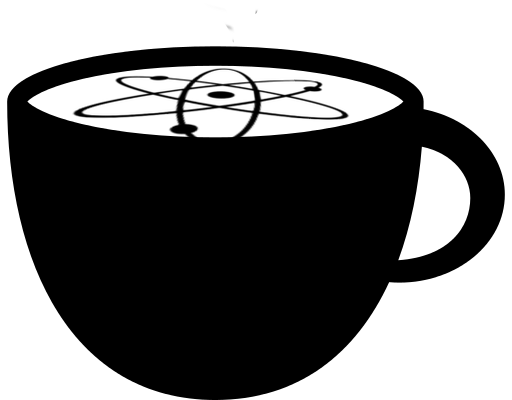
\includegraphics[height=0.5\textheight]{./images/pyrk.png}
                       \caption{Special purpose reactor kinetics python tool
                       (https://github.com/pyrk/pyrk) \cite{huff_pyrk:_2015}. 
                       Research software for simple PRKE: \emph{caveat emptor.}}
               \end{figure}

               \begin{itemize}
                       \item Multiple precursor groups ($j$ groups)
                       \item Multiple decay heat groups ($k$ groups)
                       \item Lumped Parameter thermal hydraulics model
                       \item Optional 1-D conduction in pebble fuel compacts
                       \item Object-oriented, geometry and material agnostic framework
               \end{itemize}
\end{frame}


%------------------------------------------------------------------------------------
\begin{frame}
        \frametitle{Point Reactor Kinetics}
        \begin{align}
    p &= \mbox{ reactor power }\\
    \rho(t,&T_{fuel},T_{cool},T_{mod}, T_{refl}) = \mbox{ reactivity}\\
    \beta &= \mbox{ fraction of neutrons that are delayed}\\
    \beta_j &= \mbox{ fraction of delayed neutrons from precursor group j}\\
    \zeta_j &= \mbox{ concentration of precursors of group j}\\
    \lambda_{d,j} &= \mbox{ decay constant of precursor group j}\\
    \Lambda &= \mbox{ mean generation time }\\
    \omega_k &= \mbox{ decay heat from FP group k}\\
    \kappa_k &= \mbox{ heat per fission for decay FP group k}\\
    \lambda_{FP,k} &= \mbox{ decay constant for decay FP group k}\\
    T_i &= \mbox{ temperature of component i}
\end{align}

\end{frame}

%------------------------------------------------------------------------------------
\begin{frame}
\frametitle{Point Reactor Kinetics}
\begin{equation}
\frac{d}{dt}\left[
    \begin{array}{c}
      p\\
      \zeta_1\\
      .\\
      \zeta_j\\
      .\\
      \zeta_J\\
      \omega_1\\
      .\\
      \omega_k\\
      .\\
      \omega_K\\
      T_{i}\\
      .\\
      T_{I}\\
    \end{array}
    \right]
    =
    \left[
      \begin{array}{ c }
        \frac{\rho(t,T_{i},\cdots)-\beta}{\Lambda}p +
        \displaystyle\sum^{j=J}_{j=1}\lambda_{d,j}\zeta_j\\
        \frac{\beta_1}{\Lambda} p - \lambda_{d,1}\zeta_1\\
        .\\
        \frac{\beta_j}{\Lambda}p-\lambda_{d,j}\zeta_j\\
        .\\
        \frac{\beta_J}{\Lambda}p-\lambda_{d,J}\zeta_J\\
        \kappa_1p - \lambda_{FP,1}\omega_1\\
        .\\
        \kappa_kp - \lambda_{FP,k}\omega_k\\
        .\\
        \kappa_{k p} - \lambda_{FP,k}\omega_{k}\\
        f_{i}(p, C_{p,i}, T_{i}, \cdots)\\
        .\\
        f_{I}(p, C_{p,I}, T_{I}, \cdots)\\
      \end{array}
      \right]
\end{equation}
\end{frame}

%------------------------------------------------------------------------------------
\begin{frame}
        \frametitle{Lumped Parameter Heat Transfer}

The heat flow out of body $i$ is the sum of surface heat flow by conduction,
convection, radiation, and other mechanisms to each adjacent body, $j$:
\begin{align}
Q &= Q_i + \sum_j Q_{ij}\\
  &=Q_i +  \sum_j\frac{T_{i} - T_{j}}{R_{th,ij}}\\
\dot{Q} &= \mbox{total heat flow out of body i }[J\cdot s^{-1}]\\
Q_i &= \mbox{other heat transfer, a constant }[J\cdot s^{-1}]\\
T_i &= \mbox{temperature of body i }[K]\\
T_j &= \mbox{temperature of body j }[K]\\
j &= \mbox{adjacent bodies }[-]\\
R_{th} &= \mbox{thermal resistence of the component }[K \cdot s \cdot J^{-1}].
\end{align}
\end{frame}

%------------------------------------------------------------------------------------
\begin{frame}
        \frametitle{PB-FHR Example}

               \begin{figure}[t]
                \vspace*{-0.1in}
                       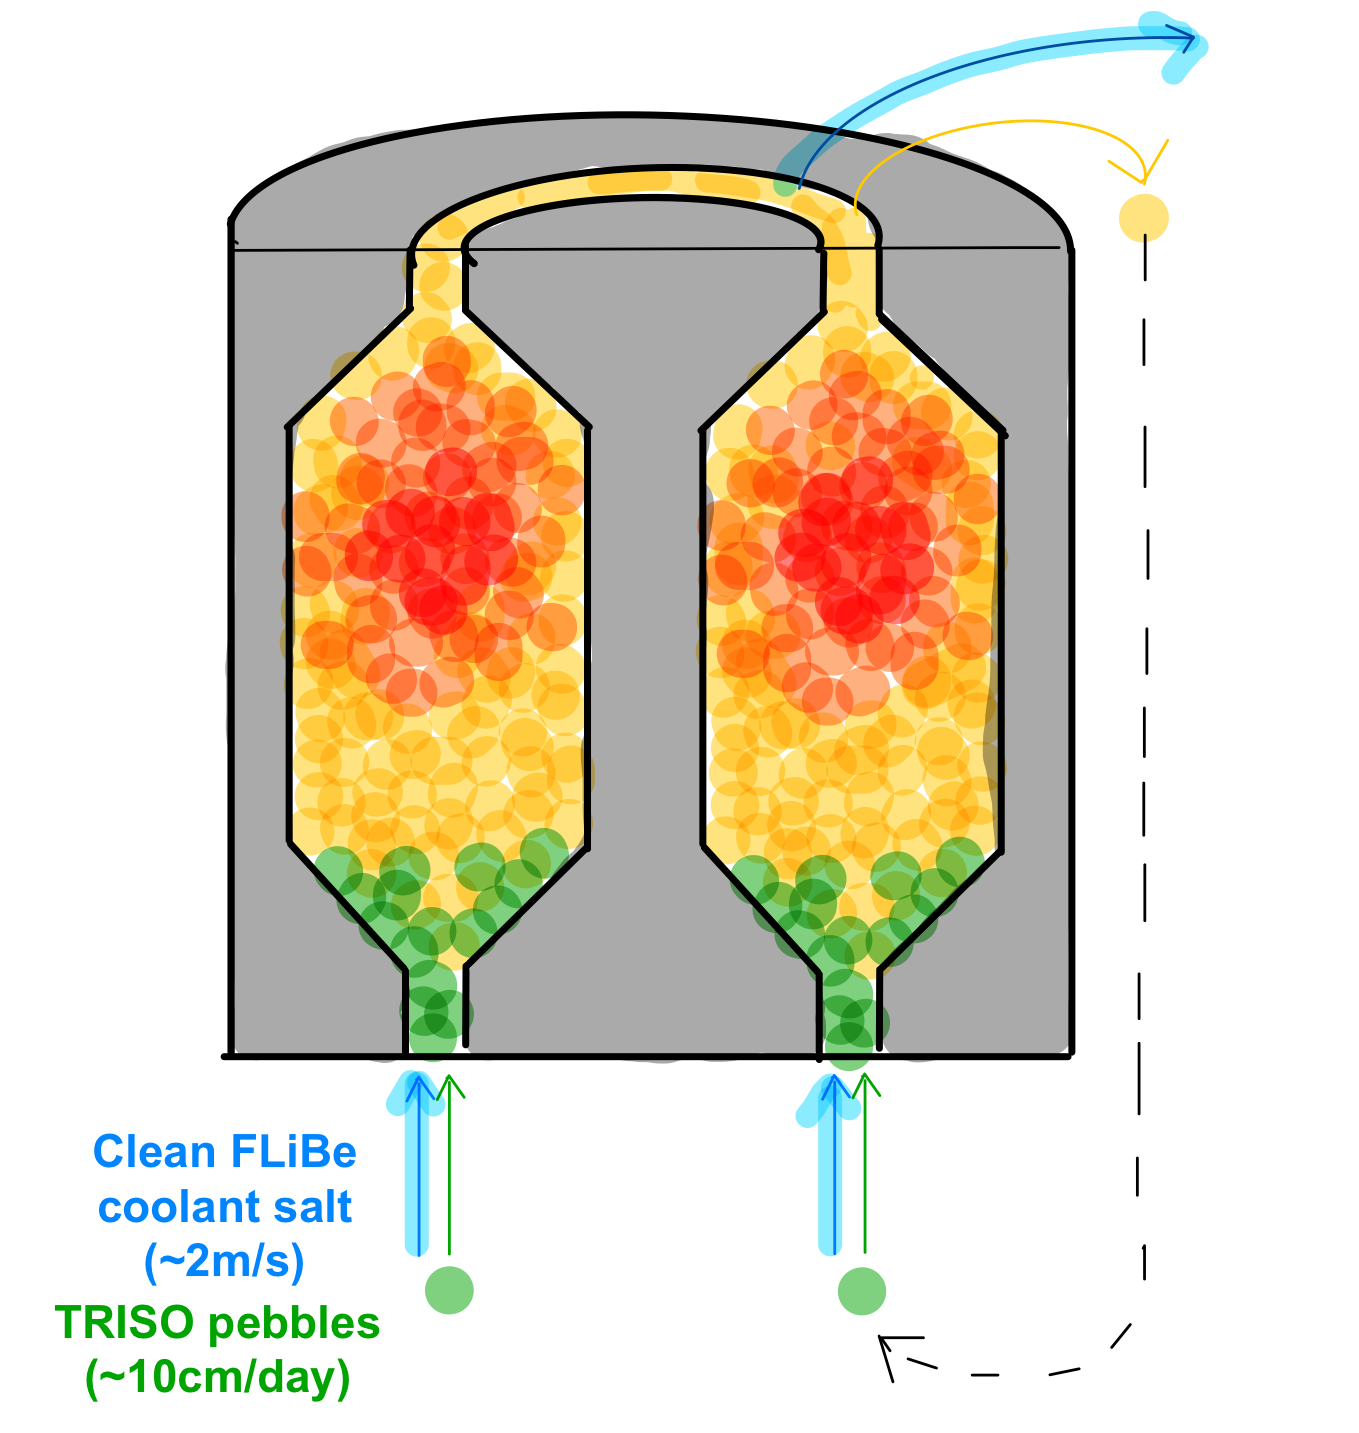
\includegraphics[height=0.5\textwidth]{./images/pbfhr-fuel-movement.png}
                       \caption{The pebble fuel can be assumed approximately 
                       stationary, as their movement is not comparable to the 
                       longest precursor decay times.}
               \end{figure}

\end{frame}


%------------------------------------------------------------------------------------
\begin{frame}
        \frametitle{Point Reactor Kinetics}

               \begin{figure}[t]
                \vspace*{-0.1in}
                       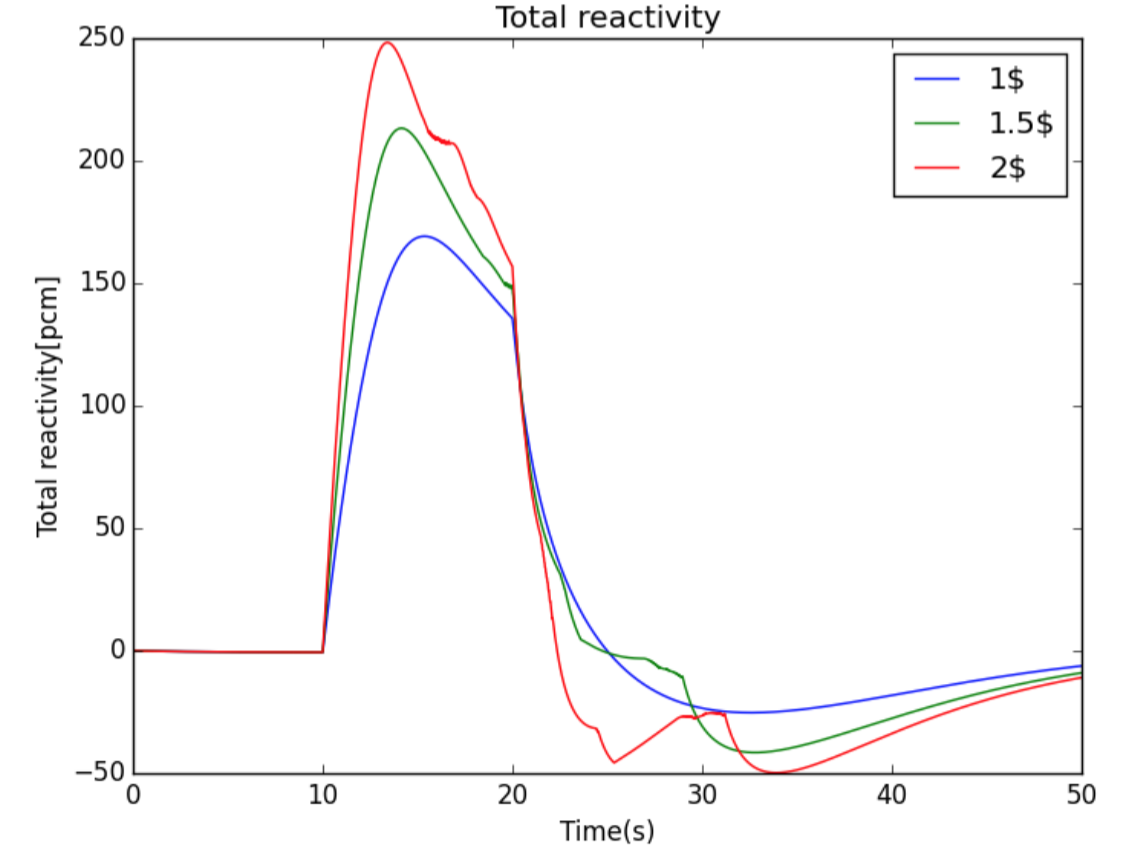
\includegraphics[height=0.5\textwidth]{./images/pbfhr-total-reactivity.png}
                       \caption{Total reactivity during ramped reactivity 
                       insertion as a function of inserted reactivity
                       \cite{wang_coupled_2016}.}
               \end{figure}

\end{frame}



%------------------------------------------------------------------------------------
\begin{frame}
        \frametitle{PB-FHR Example}

               \begin{figure}[t]
                \vspace*{-0.1in}
                       \hspace*{-0.3in}
                       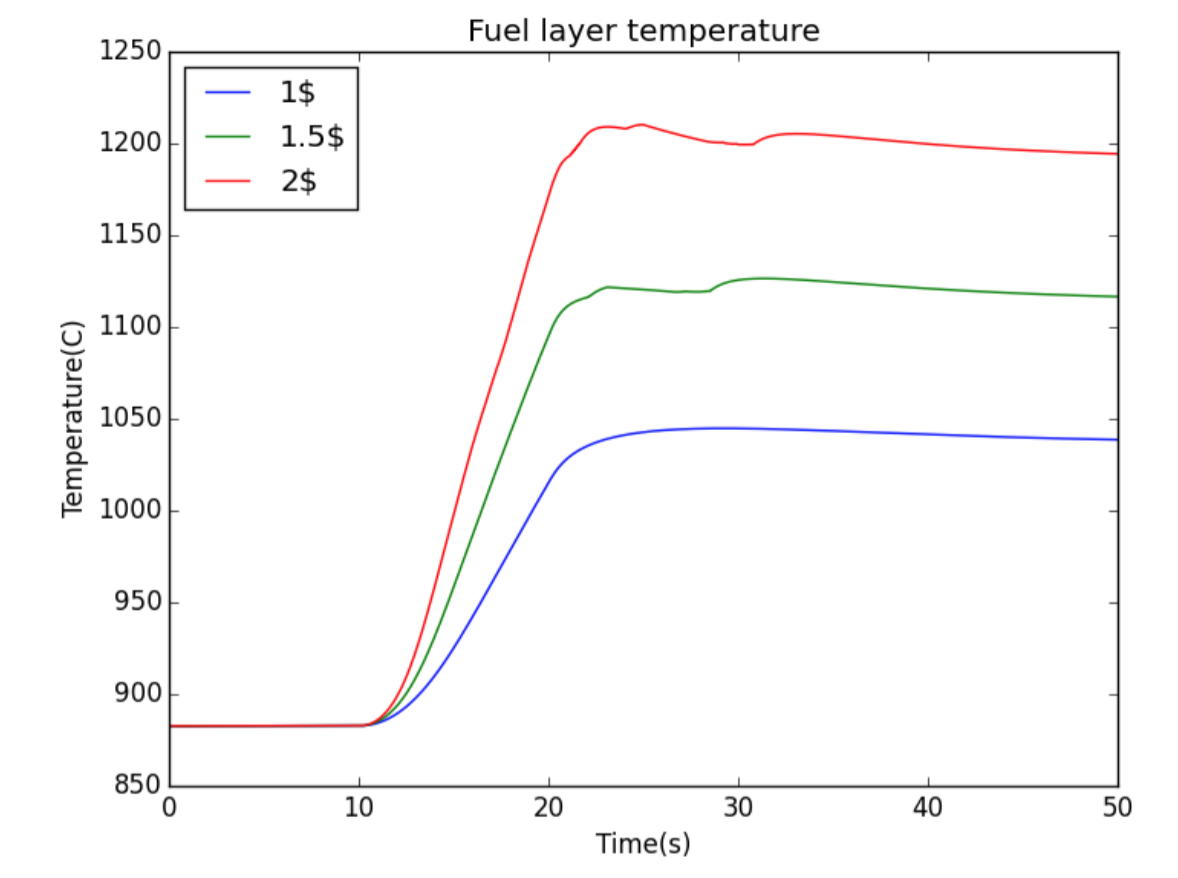
\includegraphics[height=0.3\textwidth]{./images/pbfhr-fuel-temp.png}
                       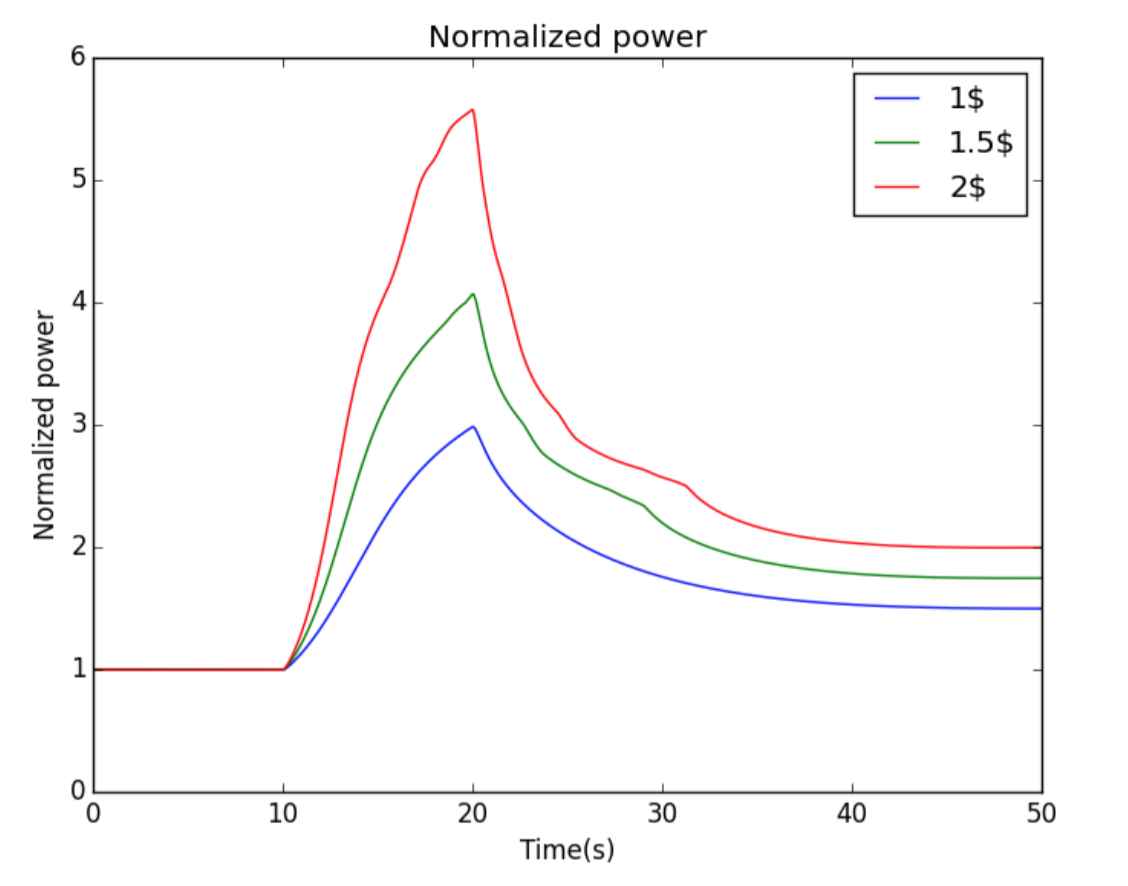
\includegraphics[height=0.3\textwidth]{./images/pbfhr-avg-pow.png}
                       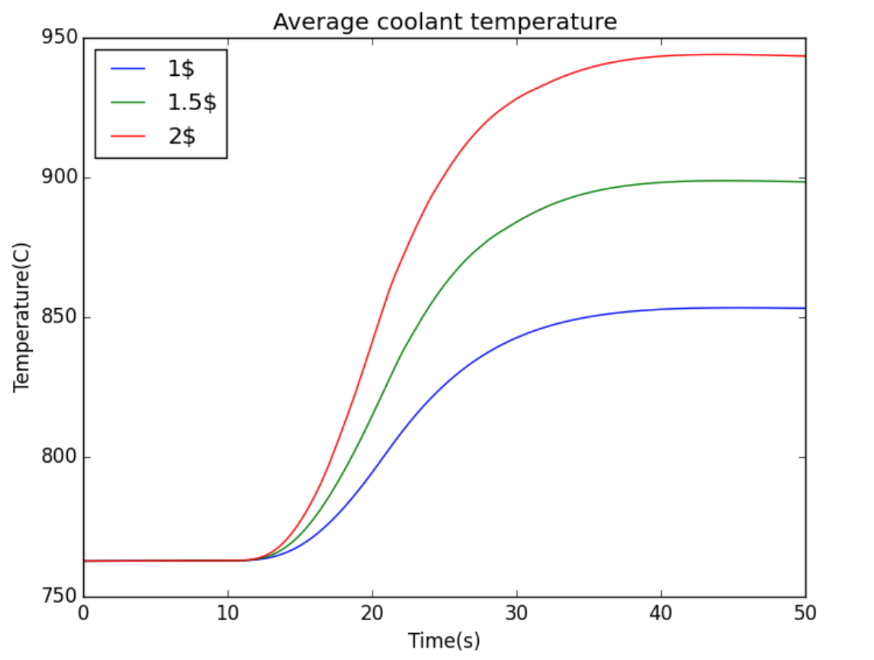
\includegraphics[height=0.3\textwidth]{./images/pbfhr-coolant-temp.png}
                       \caption{Average fuel temperature (left) and average 
                       normalized core power (right) during a ramp reactivity 
                       insertion in the PB-FHR \cite{wang_coupled_2016}.}
               \end{figure}

\end{frame}


%------------------------------------------------------------------------------------
\begin{frame}
        \frametitle{Point Reactor Kinetics}

               \begin{figure}[t]
                \vspace*{-0.1in}
                       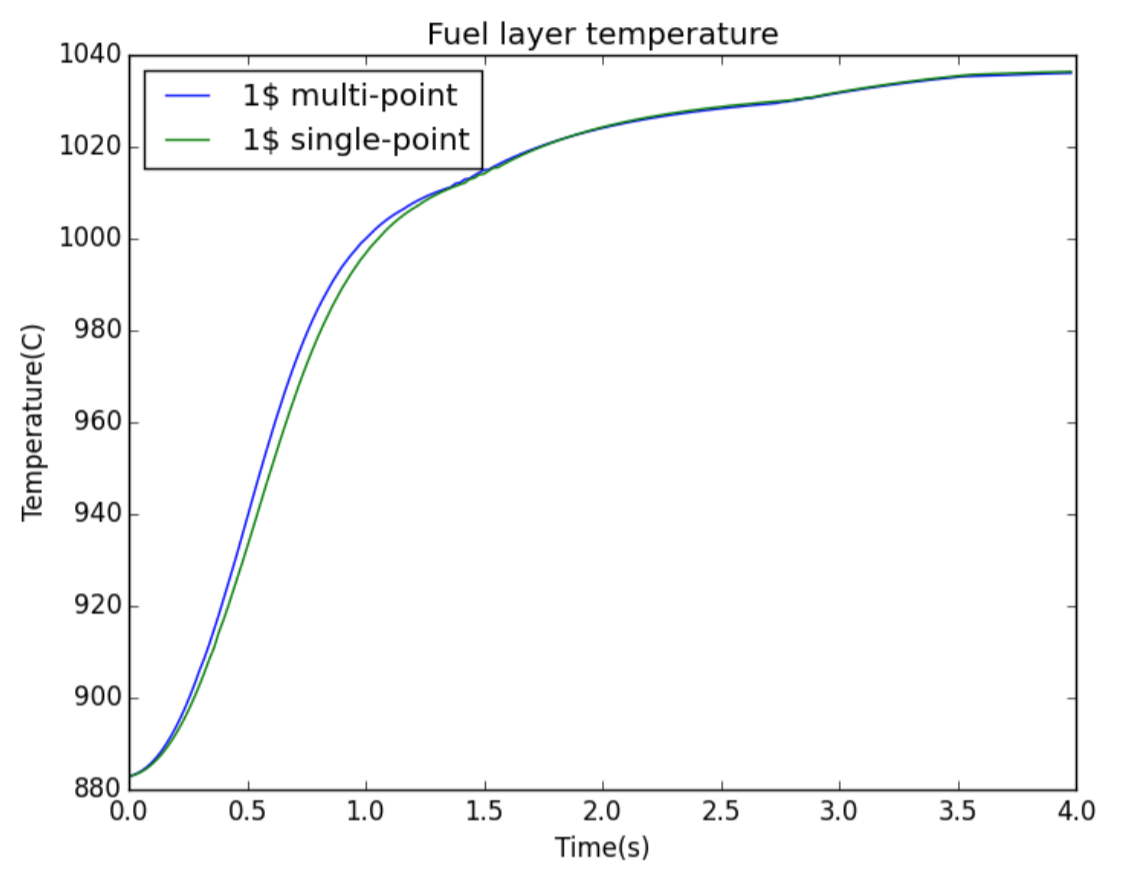
\includegraphics[height=0.5\textwidth]{./images/pbfhr-multi-single-point.png}
                       \caption{Fuel temperature rise following 1\$ ramp 
                       reactivity insertion, calculated with multipoint and 
                       single point kinetics in PyRK \cite{wang_coupled_2016}.}
               \end{figure}

\end{frame}
